\documentclass[11pt, a4paper]{article}

% --- Essential Packages ---
\usepackage[utf8]{inputenc}
\usepackage[T1]{fontenc}
\usepackage{lmodern} % Or other modern font like 'kpfonts', 'tgtermes'
\usepackage[margin=2.5cm]{geometry} % Adjust margins as needed
\usepackage{amsmath, amssymb} % For math symbols if needed (good practice)
\usepackage{graphicx} % To include images (placeholder included)
\usepackage[svgnames, table]{xcolor} % For colors, needed by hyperref and listings
\usepackage{enumitem} % For customized lists
\usepackage{booktabs} % For professional tables
\usepackage{microtype} % Improves typography subtly
\usepackage{ragged2e} % For better justification control if needed
% \usepackage{lipsum} % For dummy text (remove or comment out in final version)

% --- Hyperlinking and References ---
\usepackage{hyperref}
\hypersetup{
    colorlinks=true,
    linkcolor=Blue,
    citecolor=Green,
    urlcolor=NavyBlue,
    pdftitle={A Detailed Explanation of Knowledge Graphs},
    pdfauthor={AI Assistant},
    pdfsubject={Knowledge Representation},
    pdfkeywords={Knowledge Graph, Semantic Web, Linked Data, RDF, SPARQL, Ontology},
    % bookmarks=true, % Keep only one bookmarks entry
    bookmarksopen=true,
}
% --- Bibliography Setup (Using biblatex) ---
% Make sure references.bib is in the same folder
\usepackage[backend=biber, style=ieee, sorting=nyt]{biblatex} % Modern bibliography
\addbibresource{references.bib} % Link to your .bib file

% --- Code Listings ---
\usepackage{listings}
\definecolor{codegreen}{rgb}{0,0.6,0}
\definecolor{codegray}{rgb}{0.5,0.5,0.5}
\definecolor{codepurple}{rgb}{0.58,0,0.82}
\definecolor{backcolour}{rgb}{0.98,0.98,0.98}

\lstdefinestyle{sparqlstyle}{
    backgroundcolor=\color{backcolour},
    commentstyle=\color{codegreen},
    keywordstyle=\color{magenta},
    numberstyle=\tiny\color{codegray},
    stringstyle=\color{codepurple},
    basicstyle=\footnotesize\ttfamily,
    breakatwhitespace=false,
    breaklines=true,
    captionpos=b,
    keepspaces=true,
    numbers=left,
    numbersep=5pt,
    showspaces=false,
    showstringspaces=false,
    showtabs=false,
    tabsize=2,
    language=SQL, % SPARQL is SQL-like, good enough for basic highlighting
    morekeywords={PREFIX, SELECT, WHERE, FILTER, OPTIONAL, UNION, GRAPH, DISTINCT, ASK, CONSTRUCT, DESCRIBE, LIMIT, OFFSET, ORDER, BY, ASC, DESC, STR, LANG, DATATYPE, IRI, URI, BNODE, REGEX, BOUND, SAMETERM, ISIRI, ISBLANK, ISLITERAL, a, rdfs:label} % Add SPARQL keywords, included rdfs:label
}
\lstset{style=sparqlstyle}

% --- TikZ for Diagrams ---
\usepackage{tikz}
\usetikzlibrary{arrows.meta, shapes, positioning, calc}
\usepackage{caption} % Needed for \captionof

% --- Document Information ---
\title{\Huge A Detailed Explanation of Knowledge Graphs}
\author{Generated by AI Assistant}
\date{March 30, 2025} % Changed from \today to match original PDF date

% --- START DOCUMENT ---
\begin{document}

\maketitle
\RaggedRight % Often better for readability than full justification

\begin{abstract}
\noindent Knowledge Graphs (KGs) have emerged as a powerful paradigm for organizing, managing, and integrating information by representing knowledge as a network of interconnected entities and their relationships. This document provides a detailed exploration of Knowledge Graphs, covering their fundamental concepts, core components (nodes, edges, triples), underlying technologies (RDF, OWL, URIs), different types, the complex creation lifecycle (extraction, integration, storage), querying mechanisms like SPARQL, diverse applications across industries, inherent benefits, and significant challenges. The goal is to offer a comprehensive understanding of what KGs are, how they work, and why they are increasingly vital in the age of big data and artificial intelligence.
\end{abstract}

\tableofcontents
\clearpage

% --- SECTIONS ---

\section{Introduction: What is a Knowledge Graph?}
\label{sec:introduction}

At its core, a Knowledge Graph (KG) is a structured representation of knowledge modeled as a graph. Instead of storing data in tables with rows and columns, a KG stores information as a network of:
\begin{itemize}
    \item \textbf{Entities} (Nodes or Vertices): Representing real-world objects, concepts, events, or abstract ideas (e.g., "Paris", "Eiffel Tower", "Person", "Company").
    \item \textbf{Relationships} (Edges or Links): Representing the connections or interactions between entities (e.g., "is located in", "was designed by", "works for").
    \item \textbf{Attributes/Properties} (Often associated with nodes): Representing specific characteristics of entities (e.g., the population of "Paris", the height of the "Eiffel Tower").
\end{itemize}

Think of it as a way to connect pieces of information contextually, much like the human brain links concepts. This structure allows for more flexible querying and inference compared to traditional relational databases. KGs are often built upon Semantic Web technologies like the Resource Description Framework (RDF) and Web Ontology Language (OWL), enabling machine-readable semantics and interoperability \cite{BernersLee2001}. They aim to capture not just data, but the *meaning* and *context* surrounding that data.

The rise of KGs is driven by the need to handle vast amounts of heterogeneous data, break down data silos, and power more intelligent applications, from search engines \cite{GoogleKG} to sophisticated AI systems.

\section{Core Components and Concepts}
\label{sec:core_components}

Understanding KGs requires familiarity with several key building blocks:

\subsection{Nodes (Entities)}
\label{subsec:nodes}
Nodes represent the primary subjects or objects of interest. They can be concrete (e.g., \textit{Leonardo da Vinci}, \textit{Mona Lisa}) or abstract (e.g., \textit{Art}, \textit{Renaissance}). Each significant entity in a KG is typically assigned a Unique Resource Identifier (URI), often an HTTP URI, to ensure global uniqueness and allow linking across different datasets (a core principle of Linked Data).

\subsection{Edges (Relationships and Properties)}
\label{subsec:edges}
Edges connect nodes, defining how entities relate to each other. These relationships are directional and labeled with predicates (also often identified by URIs). For example, an edge might represent the relationship \texttt{painted} connecting \textit{Leonardo da Vinci} to \textit{Mona Lisa}. Edges can also represent attributes or properties of a node, linking an entity node to a literal value node (e.g., linking \textit{Mona Lisa} to the literal "1503" via the edge \texttt{creationDate}).

\subsection{Triples (Subject-Predicate-Object)}
\label{subsec:triples}
The fundamental unit of data in many KGs, particularly those based on RDF, is the \textbf{triple}. It consists of:
\begin{itemize}
    \item \textbf{Subject:} An entity (URI or blank node).
    \item \textbf{Predicate:} A relationship or property (URI).
    \item \textbf{Object:} Another entity (URI or blank node) or a literal value (string, number, date).
\end{itemize}
For example: `(<http://example.org/Leonardo>, <http://example.org/painted>, <http://example.org/MonaLisa>)` or `(<http://example.org/MonaLisa>, <http://example.org/creationDate>, "1503"^^xsd:gYear)`. A KG is essentially a large collection of such triples.

\subsection{Schema and Ontology}
\label{subsec:schema_ontology}
While some KGs can be schema-agnostic, many benefit from an associated \textbf{schema} or \textbf{ontology}. This provides a formal description of the types of entities (classes) and relationships (properties) allowed in the graph, along with rules, constraints, and hierarchies (e.g., defining that a `Painter` is a type of `Artist`, which is a type of `Person`). Ontologies, often defined using standards like RDFS (RDF Schema) or OWL (Web Ontology Language), add richer semantics, enabling consistency checking and logical reasoning (inference) over the graph data \cite{OWL2Overview}.

\subsection{Unique Resource Identifiers (URIs)}
\label{subsec:uris}
URIs are crucial for uniquely identifying entities and predicates, especially in open KGs designed for linking across the web. Using HTTP URIs allows these identifiers to be dereferenceable, potentially providing more information about the resource. Examples include URIs from DBpedia (e.g., `http://dbpedia.org/resource/Paris`) or Wikidata (e.g., `http://www.wikidata.org/entity/Q90`).

\subsection{Visual Example}
\label{subsec:visual_example}
The following diagram illustrates a small segment of a hypothetical KG:

\begin{center}
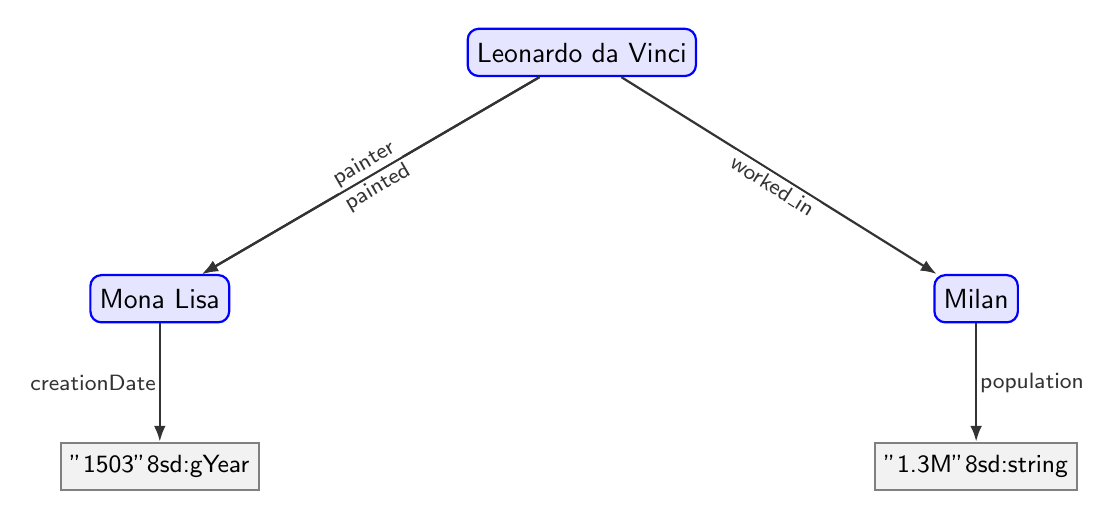
\begin{tikzpicture}[
    node distance=2.5cm and 3cm,
    entity/.style={rectangle, rounded corners, draw=Blue, thick, fill=Blue!10, minimum size=6mm, font=\sffamily},
    literal/.style={rectangle, draw=Gray, thick, fill=Gray!10, minimum size=6mm, font=\sffamily\small},
    edge_lbl/.style={midway, fill=white, inner sep=1pt, font=\sffamily\footnotesize\color{black!70}},
    arrow/.style={-{Latex[length=2mm]}, thick, color=black!80}
    ]

    % Nodes
    \node[entity] (leo) {Leonardo da Vinci};
    \node[entity, below left=of leo] (mona) {Mona Lisa};
    \node[entity, below right=of leo] (milan) {Milan};
    \node[literal, below=1.5cm of mona] (date) {"1503"^^xsd:gYear};
    \node[literal, below=1.5cm of milan] (pop) {"1.3M"^^xsd:string};

    % Edges
    \draw[arrow] (leo) -- (mona) node[edge_lbl, below, sloped] {painted};
    \draw[arrow] (leo) -- (milan) node[edge_lbl, below, sloped] {worked\_in};
    \draw[arrow] (mona) -- (date) node[edge_lbl, left] {creationDate};
    \draw[arrow] (milan) -- (pop) node[edge_lbl, right] {population};
    \draw[arrow, bend left=20] (leo) -- (mona) node[edge_lbl, above, sloped] {painter}; % Example inverse relationship (semantic, maybe not explicit edge) - kept leo->mona for consistency
\end{tikzpicture}
\captionof{figure}{A simple visual representation of KG triples.}
\label{fig:kg_example}
\end{center}

\section{Types of Knowledge Graphs}
\label{sec:types}

Knowledge Graphs can be categorized based on various criteria:

\subsection{Scope}
\label{subsec:scope}
\begin{itemize}
    \item \textbf{General / Cross-Domain KGs:} Aim to cover a broad range of topics and entities from the real world. Examples include DBpedia \cite{DBpedia}, Wikidata, YAGO, and the Google Knowledge Graph \cite{GoogleKG}. They often integrate data from multiple open sources like Wikipedia.
    \item \textbf{Domain-Specific KGs:} Focus on a particular field, such as medicine (e.g., BioPortal ontologies), finance, engineering, or cultural heritage. They typically contain deeper, more specialized knowledge within their domain.
\end{itemize}

\subsection{Accessibility and Source}
\label{subsec:accessibility}
\begin{itemize}
    \item \textbf{Open KGs:} Publicly available datasets, often under open licenses, fostering collaboration and reuse (e.g., Wikidata, DBpedia \cite{DBpedia}).
    \item \textbf{Enterprise KGs:} Proprietary graphs built within organizations to manage internal knowledge, integrate diverse data sources (databases, documents, logs), and power internal applications. These are typically not public.
\end{itemize}

\section{Knowledge Graph Creation Lifecycle}
\label{sec:creation_lifecycle}

Building a KG is a complex, iterative process involving several stages:

\subsection{Knowledge Extraction}
\label{subsec:extraction}
This involves identifying and extracting entities, relationships, and attributes from various data sources:
\begin{itemize}
    \item \textbf{Structured Sources:} Mapping relational databases or spreadsheets to the KG's schema (e.g., using R2RML).
    \item \textbf{Semi-Structured Sources:} Parsing data from web pages (HTML tables, lists), JSON, or XML files. Web scraping and wrapper induction techniques are common.
    \item \textbf{Unstructured Sources:} Processing plain text documents (articles, reports, emails) using Natural Language Processing (NLP) techniques like Named Entity Recognition (NER) to identify entities and Relation Extraction (RE) to find relationships between them.
\end{itemize}

\subsection{Knowledge Integration and Linking}
\label{subsec:integration}
Extracted knowledge needs to be cleaned, fused, and linked:
\begin{itemize}
    \item \textbf{Entity Resolution (Disambiguation):} Identifying and merging different mentions or representations that refer to the same real-world entity (e.g., "NYC", "New York City", "Big Apple").
    \item \textbf{Schema Mapping/Alignment:} Aligning different schemas or ontologies if integrating data from multiple sources with varying structures.
    \item \textbf{Link Prediction/Inference:} Using reasoning or machine learning models to infer missing links or relationships based on existing graph patterns.
    \item \textbf{Linking to Existing KGs:} Connecting internal entities to well-known entities in public KGs (like Wikidata) to enrich the graph and improve interoperability.
\end{itemize}

\subsection{Knowledge Curation and Refinement}
\label{subsec:curation}
Ensuring the quality and accuracy of the KG:
\begin{itemize}
    \item \textbf{Validation:} Checking data against schema constraints, logical rules, or external ground truth.
    \item \textbf{Error Detection and Correction:} Identifying and fixing inconsistencies, inaccuracies, or outdated information.
    \item \textbf{Enrichment:} Adding missing attributes or relationships, often through inference or linking to external sources.
    \item \textbf{Human-in-the-Loop:} Incorporating expert feedback to validate and refine extracted or inferred knowledge.
\end{itemize}

\subsection{Knowledge Storage}
\label{subsec:storage}
Choosing the right technology to store and manage the KG:
\begin{itemize}
    \item \textbf{RDF Triple Stores:} Databases optimized for storing and querying RDF triples (e.g., Apache Jena Fuseki, Virtuoso Universal Server, GraphDB, Stardog). They typically support SPARQL querying.
    \item \textbf{Property Graph Databases:} Databases that model data as nodes, relationships, and key-value properties on both (e.g., Neo4j, ArangoDB, JanusGraph). They often use different query languages like Cypher or Gremlin. Adaptors exist to handle RDF data.
    \item \textbf{Hybrid Systems:} Solutions combining aspects of both or leveraging traditional databases with graph layers.
\end{itemize}

\section{Querying Knowledge Graphs}
\label{sec:querying}

Retrieving information from KGs often requires specialized query languages:

\subsection{SPARQL (SPARQL Protocol and RDF Query Language)}
\label{subsec:sparql}
The W3C standard query language for RDF data \cite{SPARQL11Query}. SPARQL allows users to query KGs based on graph patterns. Key query forms include:
\begin{itemize}
    \item \texttt{SELECT}: Returns data in a tabular format, similar to SQL.
    \item \texttt{CONSTRUCT}: Returns an RDF graph constructed based on query results.
    \item \texttt{ASK}: Returns true/false depending on whether a query pattern matches.
    \item \texttt{DESCRIBE}: Returns an RDF graph describing specified resources (implementation-dependent).
\end{itemize}

\begin{lstlisting}[caption={Example SPARQL query to find painters born in Italy.}, label=lst:sparql_example]
PREFIX dbo: <http://dbpedia.org/ontology/>
PREFIX dbr: <http://dbpedia.org/resource/>
PREFIX rdfs: <http://www.w3.org/2000/01/rdf-schema#>

SELECT DISTINCT ?painter ?birthPlaceName
WHERE {
  ?painter a dbo:Painter .
  ?painter dbo:birthPlace ?birthPlace .
  ?birthPlace a dbo:Country ;
              rdfs:label ?birthPlaceName .
  FILTER (LANG(?birthPlaceName) = "en" && CONTAINS(?birthPlaceName, "Italy"))
}
LIMIT 10
\end{lstlisting}

\subsection{Other Query Mechanisms}
\label{subsec:other_query}
\begin{itemize}
    \item \textbf{GraphQL:} While not specific to KGs, it's increasingly used as an API layer over KGs, providing a flexible way for applications to request exactly the data they need.
    \item \textbf{Cypher (Neo4j):} A declarative query language for property graphs, focusing on ASCII-art pattern matching.
    \item \textbf{Gremlin (Apache TinkerPop):} A graph traversal language.
    \item \textbf{Keyword Search / Natural Language Querying:} Systems built on top of KGs can translate natural language questions or keyword searches into formal graph queries.
\end{itemize}

\section{Applications of Knowledge Graphs}
\label{sec:applications}

KGs are used across a wide range of domains:

\begin{itemize}[leftmargin=*]
    \item \textbf{Semantic Search:} Powering search engines (like Google, Bing) to understand user intent better and provide direct answers or rich results (knowledge panels).
    \item \textbf{Recommender Systems:} Providing more diverse and explainable recommendations (e.g., in e-commerce, media streaming) by understanding relationships between users, items, and their attributes.
    \item \textbf{Data Integration and Master Data Management:} Creating a unified view across disparate data silos within an enterprise.
    \item \textbf{Artificial Intelligence and Machine Learning:} Providing background knowledge, context, and features for ML models, enhancing tasks like NLP, computer vision, and automated reasoning.
    \item \textbf{Question Answering and Chatbots:} Enabling systems to understand and answer complex questions by querying structured knowledge.
    \item \textbf{Life Sciences and Drug Discovery:} Integrating diverse biological data (genes, proteins, drugs, diseases) to identify potential drug targets or understand disease mechanisms.
    \item \textbf{Financial Services:} For risk analysis, fraud detection, and regulatory compliance by modeling complex relationships between entities, transactions, and regulations.
    \item \textbf{Personal Assistants:} Enabling devices like Alexa or Siri to understand commands and retrieve relevant information.
\end{itemize}

\section{Benefits of Using Knowledge Graphs}
\label{sec:benefits}

Adopting a KG approach offers several advantages:

\begin{itemize}
    \item \textbf{Contextual Understanding:} Represents data with its meaning and relationships, enabling deeper insights.
    \item \textbf{Data Integration:} Breaks down silos by providing a unified model for heterogeneous data sources.
    \item \textbf{Flexibility and Evolvability:} Graph models are generally easier to extend and modify than rigid relational schemas.
    \item \textbf{Enhanced Data Discovery:} Allows users to explore connections and discover non-obvious relationships.
    \item \textbf{Foundation for AI:} Provides structured knowledge crucial for reasoning, explainability, and advanced AI applications.
    \item \textbf{Improved Data Quality:} The process of KG creation often involves explicit steps for cleaning, validation, and disambiguation.
\end{itemize}

\section{Challenges in Knowledge Graph Implementation}
\label{sec:challenges}

Despite the benefits, building and maintaining KGs presents significant challenges:

\begin{itemize}
    \item \textbf{Scalability:} Handling the sheer volume, velocity, and variety of data can be demanding for storage, querying, and reasoning.
    \item \textbf{Data Quality and Accuracy:} Ensuring the correctness, completeness, and consistency of the knowledge is difficult, especially when extracting from noisy or unstructured sources.
    \item \textbf{Creation Cost and Complexity:} The extraction, integration, and curation processes can be resource-intensive and require specialized expertise.
    \item \textbf{Maintenance and Evolution:} KGs need to be continuously updated as the underlying world knowledge changes, which can be complex to manage.
    \item \textbf{Ambiguity and Disambiguation:} Resolving entity and relation ambiguity accurately remains a hard problem.
    \item \textbf{Query Complexity:} Formulating complex queries (especially in SPARQL) can have a steep learning curve. Performance optimization for complex queries is also challenging.
\end{itemize}

\section{Future Directions}
\label{sec:future}

The field of Knowledge Graphs is rapidly evolving:
\begin{itemize}
    \item \textbf{Automation:} Increased use of ML and LLMs to automate KG construction, enrichment, and maintenance.
    \item \textbf{Neuro-Symbolic AI:} Combining KGs (symbolic knowledge) with deep learning (sub-symbolic patterns) for more robust and explainable AI.
    \item \textbf{Explainability:} Using KGs to provide explanations for AI model predictions or decisions.
    \item \textbf{Real-time KGs:} Developing systems that can update and reason over knowledge streams in real-time.
    \item \textbf{KG Embeddings:} Representing KG components as vectors for use in downstream ML tasks, while exploring ways to retain interpretability.
    \item \textbf{Integration with Large Language Models (LLMs):} Using KGs to ground LLMs in factual knowledge (e.g., Retrieval-Augmented Generation - RAG) and using LLMs to help build and query KGs.
\end{itemize}

\section{Conclusion}
\label{sec:conclusion}

Knowledge Graphs represent a fundamental shift in how we structure, integrate, and utilize information. By focusing on the relationships and context surrounding data, they provide a powerful foundation for tackling complex data challenges and building more intelligent, context-aware applications. While challenges remain, particularly concerning scale and quality, the ongoing advancements in AI, NLP, and database technologies continue to drive the adoption and sophistication of KGs, making them an indispensable tool for knowledge representation and management in the modern data landscape.

\clearpage

% --- Bibliography using biblatex ---
% The heading=bibintoc option adds the References section to the Table of Contents
\printbibliography[heading=bibintoc]

\end{document}
% --- END DOCUMENT ---